\documentclass[12pt,addpoints,answers]{evalua}
\grado{2$^\circ$ de Secundaria}
\cicloescolar{2024-2025}
\materia{Matemáticas 2}
\unidad{2}
\title{Examen de {\color{brown}recuperación} de la Unidad}
\aprendizajes{\small%
      \item Formula expresiones de primer grado para representar propiedades (perímetros y áreas) de figuras geométricas y verifica equivalencia de expresiones, tanto algebraica como geométricamente (análisis de las figuras).
      \item Construye polígonos regulares a partir de algunas medidas (lados, apotema, diagonales, etcétera).
      \item Descompone figuras en otras para calcular su área.
      \item Calcula el perímetro y el área de polígonos regulares y del círculo a partir de diferentes datos.
}  
\author{Prof.: Julio César Melchor Pinto}
\begin{document}%
\begin{multicols}{2}
	\include*{../blocks/block002}
	\include*{../blocks/block035c}
	\include*{../blocks/block003}
	\include*{../blocks/block035b}
\end{multicols}
\begin{questions}
	% \newpage
	\question[6]{Encuentra el \textbf{perímetro} y el \textbf{área} de los siguientes círculos:

		\begin{multicols}{3}
			\begin{parts}
				% \part 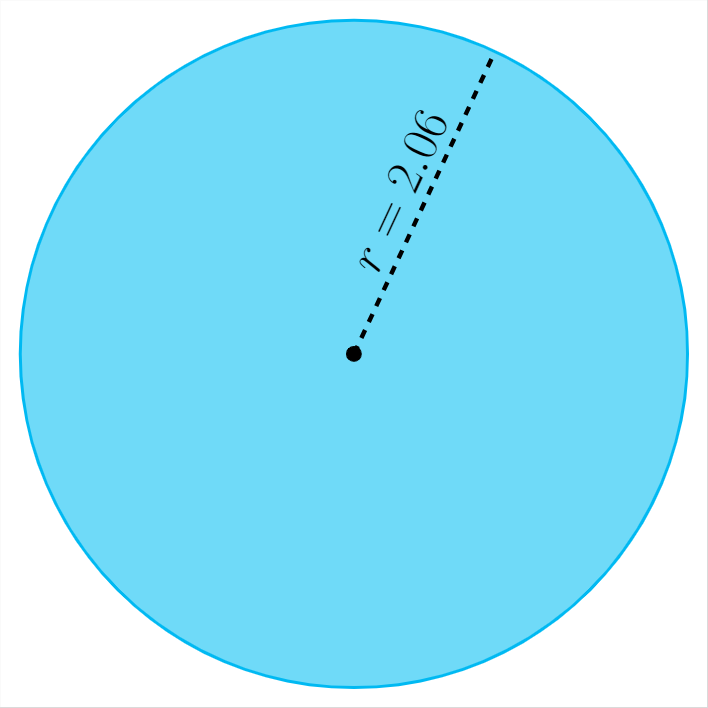
\includegraphics[width=0.85\linewidth]{mex_0001.png}\\
				% Perímetro: \fillin[][0.3in] \quad Área: \fillin[][0.3in]
				\part 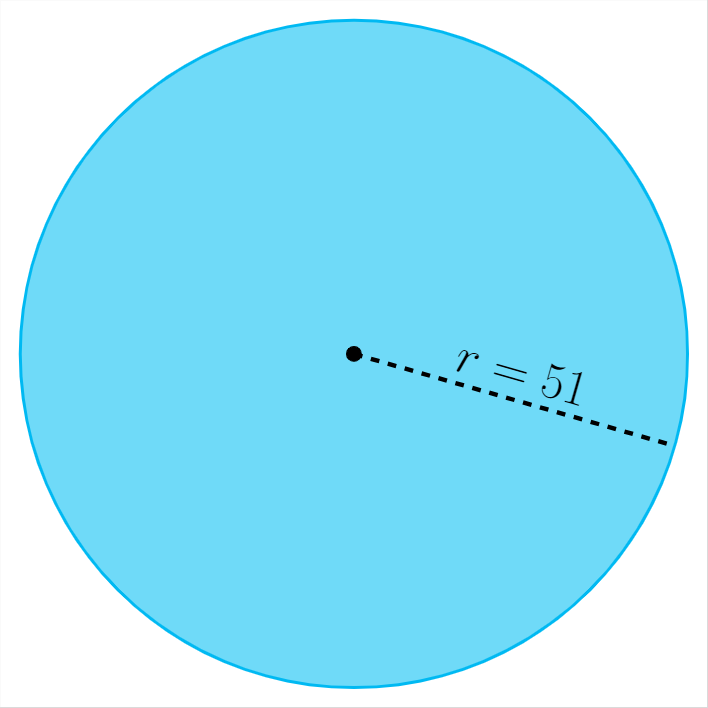
\includegraphics[width=0.85\linewidth]{mex_0002.png}\\

				Perímetro: \\
				\fillin[$P=2\pi r=2(3.14)51=320.28$][0in] \\
				Área: \\
				\fillin[$A=\pi r^2=3.14(51)^2=8167.14$][0in]

				% \part 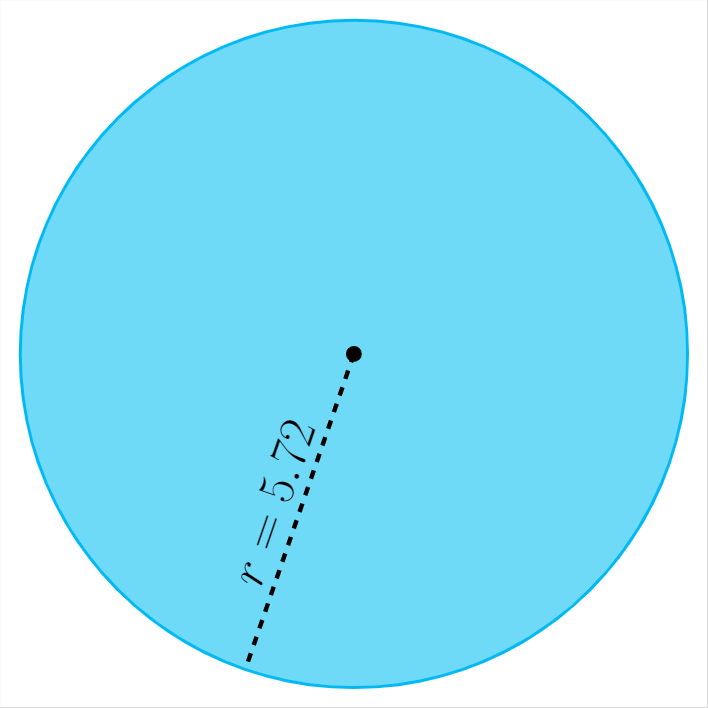
\includegraphics[width=0.85\linewidth]{mex_0003.png}\\
				% Perímetro: \fillin[][0.3in] \quad Área: \fillin[][0.3in]
				% \part 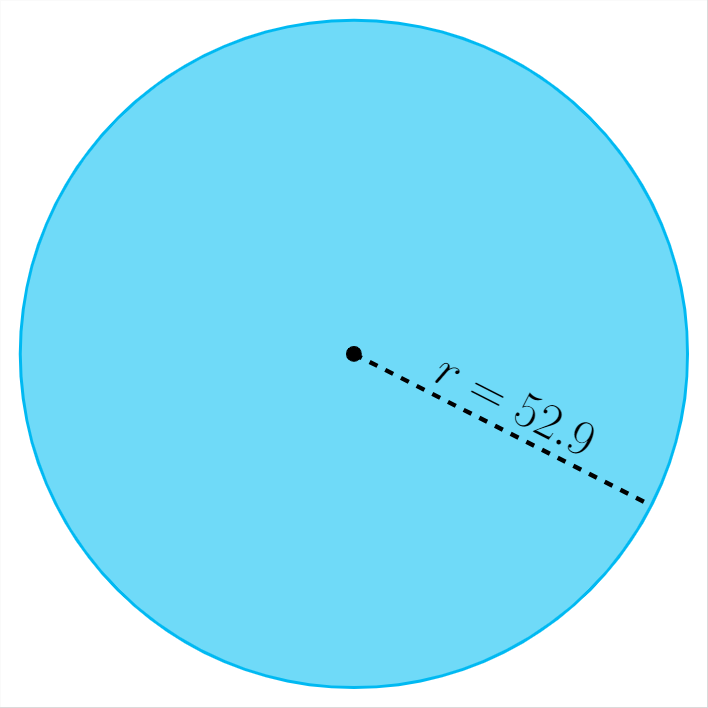
\includegraphics[width=0.85\linewidth]{mex_0004.png}\\
				% Perímetro: \fillin[][0.3in] \quad Área: \fillin[][0.3in]
				\part 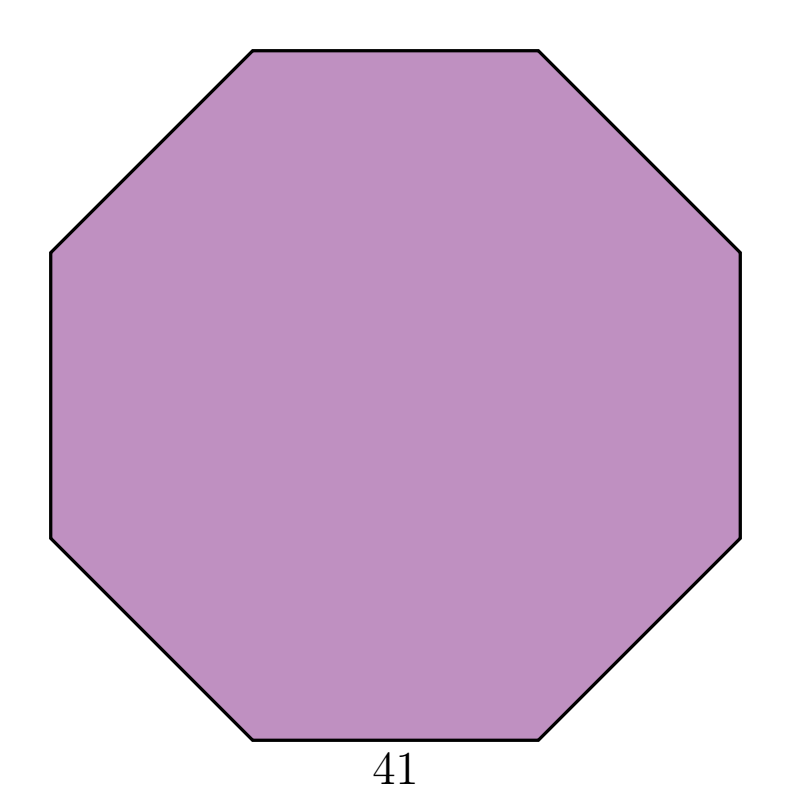
\includegraphics[width=0.85\linewidth]{mex_0005.png}\\

				Perímetro: \\
				\fillin[$P=\pi d=(3.14)14.2=44.58$][0in] \\
				Área: \\
				\fillin[$A=\pi \left(\frac{d}{2}\right)^2=3.14\left(\frac{14.2}{2}\right)^2=158.28$][0in]

				\part 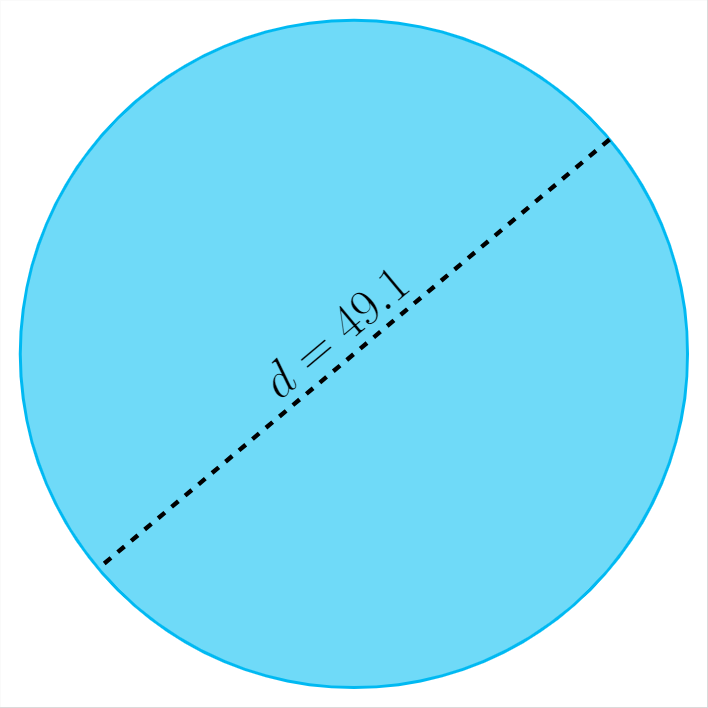
\includegraphics[width=0.85\linewidth]{mex_0009.png}\\

				Perímetro: \\
				\fillin[$P=\pi d=(3.14)49.1=154.17$][0in] \\
				Área: \\
				\fillin[$A=\pi \left(\frac{d}{2}\right)^2=3.14\left(\frac{49.1}{2}\right)^2=1892.48$][0in]
			\end{parts}
		\end{multicols}
	}

	\question[6]{Responde a las siguientes preguntas:
		\begin{multicols}{2}
			\begin{parts}
				\part La suma de los ángulos interiores de un polígono de 8 lados es:% \fillin[$1080$][0in]

				\begin{solutionbox}{1.5cm}
					\[\Sigma A_I=(n-2)(180^{\circ})=6(180^{\circ})=1080\]
				\end{solutionbox}

				\part ¿Cuánto mide el ángulo interior de un dodecágono regular?% \fillin[$150$][0in]

				\begin{solutionbox}{1.5cm}
					$A_I=\frac{(n-2)(180^{\circ})}{n} =\frac{(12-2)(180^{\circ})}{12} =150$
				\end{solutionbox}
			\end{parts}
		\end{multicols}
	}

	\question[6]{Resuelve los siguientes problemas:
		\begin{multicols}{2}
			\begin{parts}
				\part El radio de una rueda es de 32 centímetros, ¿cuántos centímetros habrá recorrido esa rueda después de haber dado 22 vueltas?
				%  \fillin[$70737.92$ cm][0in]

				\begin{solutionbox}{2cm}
					$C=2\pi r = 2\pi (32) = 201.06$ cm\\
					$22(201.06) = 70737.92$ cm
				\end{solutionbox}

				\columnbreak%


				\part Calcula el área de un parque que tiene un radio de 170 metros.
				%\fillin[$90746$ m][0in]

				\begin{solutionbox}{2cm}
					$A=\pi r^2 = \pi (170)^2 = 90746$ m$^2$
				\end{solutionbox}
			\end{parts}
		\end{multicols}
	}

	% \question[6]{Encuentra el perímetro y el área de los siguientes círculos:
	%       \begin{multicols}{3}
	%             \begin{parts}
	%                   % \part 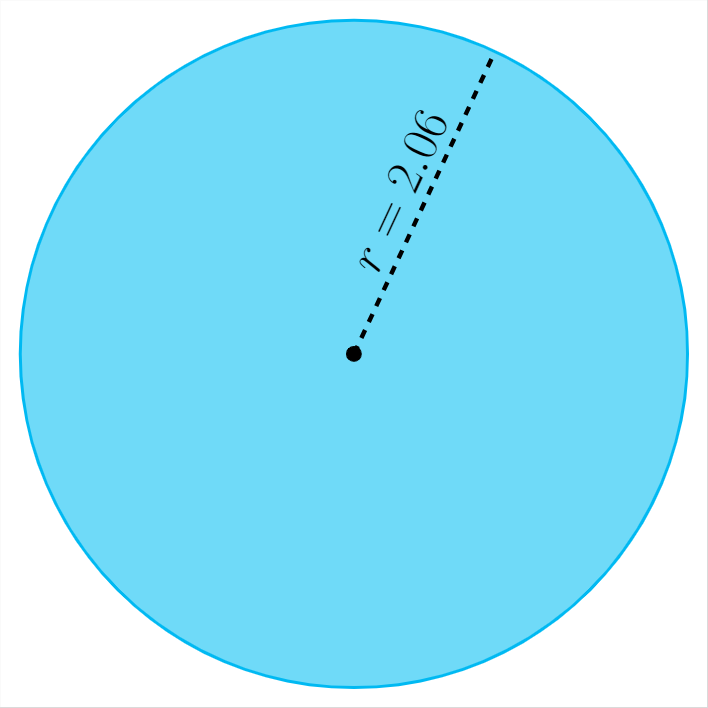
\includegraphics[width=0.85\linewidth]{mex_0001.png}\\
	%                   % Perímetro: \fillin[][0.3in] \quad Área: \fillin[][0.3in]
	%                   \part 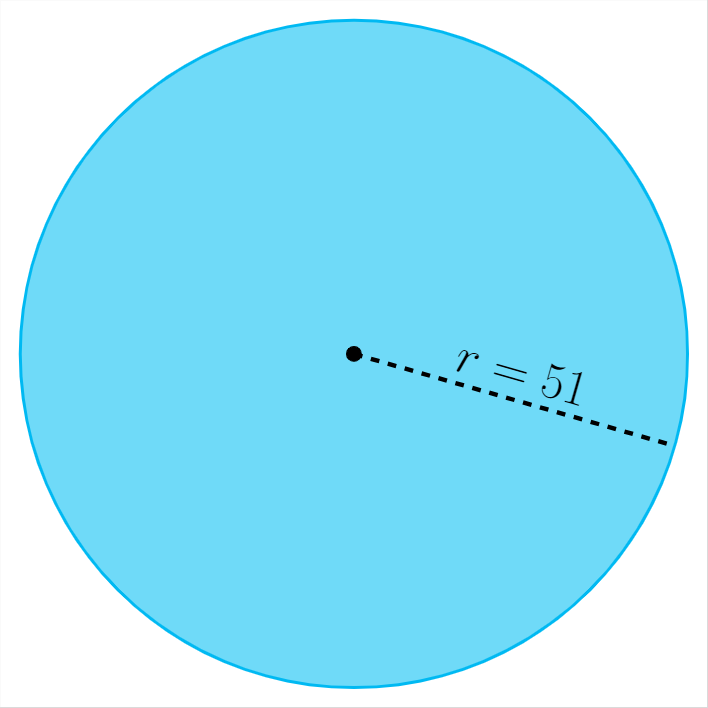
\includegraphics[width=0.85\linewidth]{mex_0002.png}\\
	%                   Perímetro: \fillin[][0.3in] \quad Área: \fillin[][0.3in]

	%                   \begin{solutionbox}{2cm}
	%                   \end{solutionbox}
	%                   % \part 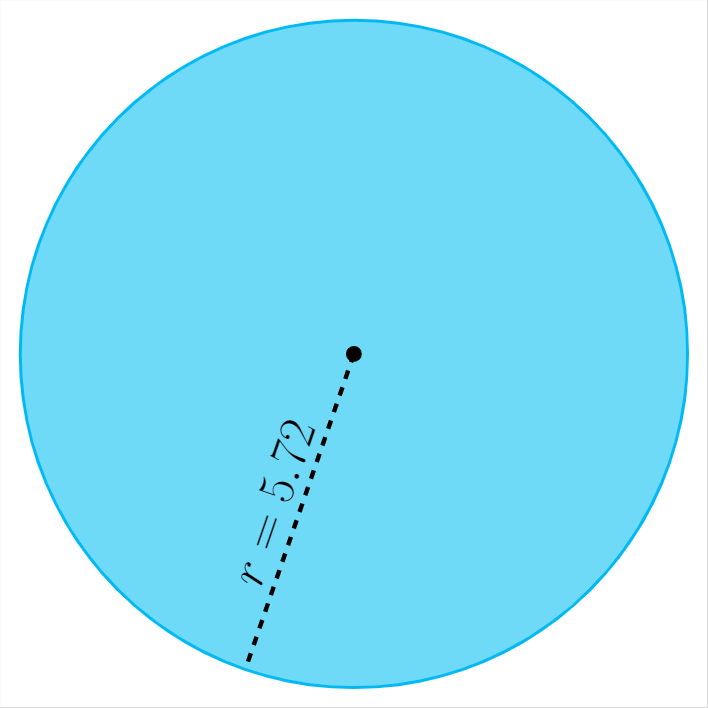
\includegraphics[width=0.85\linewidth]{mex_0003.png}\\
	%                   % Perímetro: \fillin[][0.3in] \quad Área: \fillin[][0.3in]
	%                   % \part 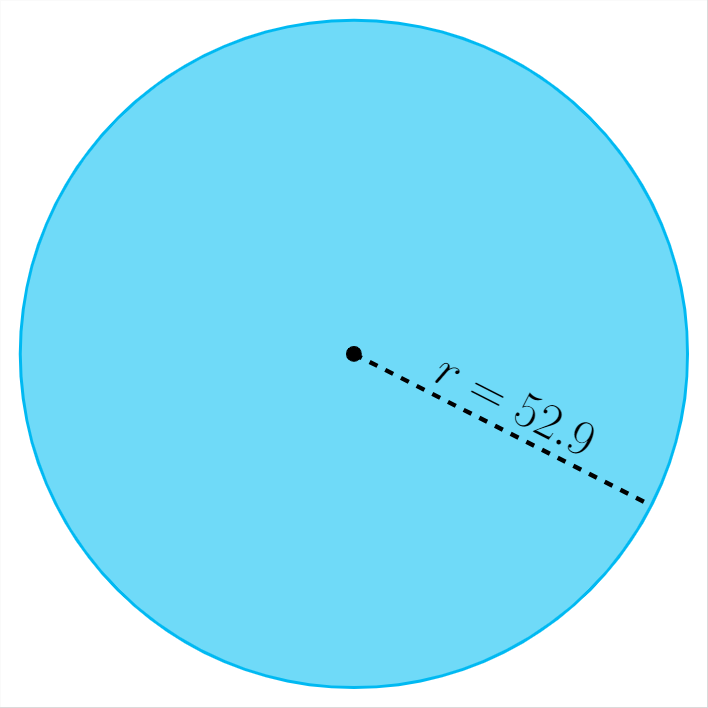
\includegraphics[width=0.85\linewidth]{mex_0004.png}\\
	%                   % Perímetro: \fillin[][0.3in] \quad Área: \fillin[][0.3in]
	%                   \part 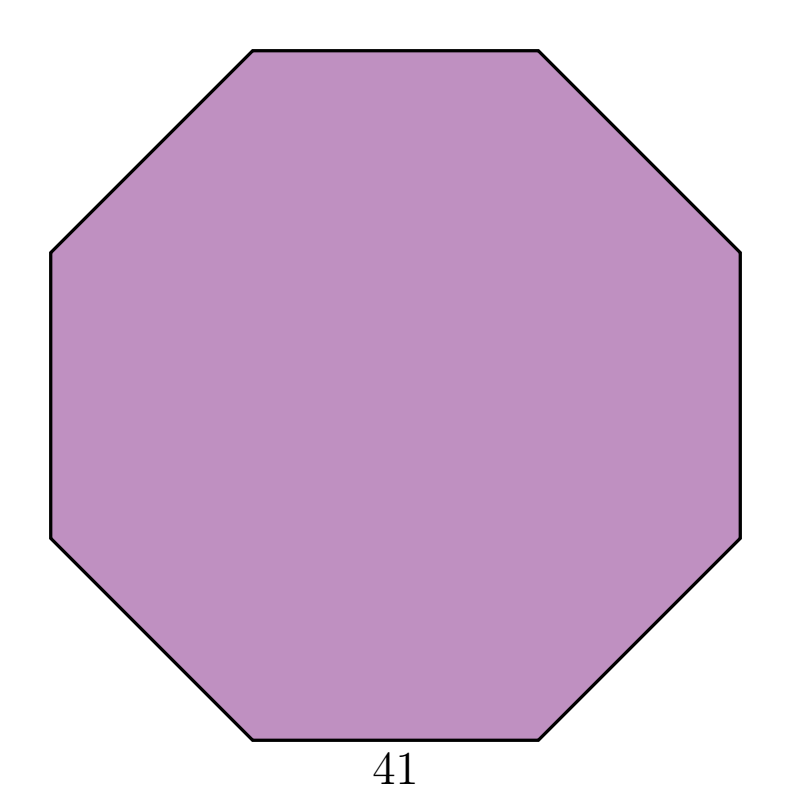
\includegraphics[width=0.85\linewidth]{mex_0005.png}\\
	%                   Perímetro: \fillin[][0.3in] \quad Área: \fillin[][0.3in]

	%                   \begin{solutionbox}{2cm}
	%                   \end{solutionbox}
	%                   % \part 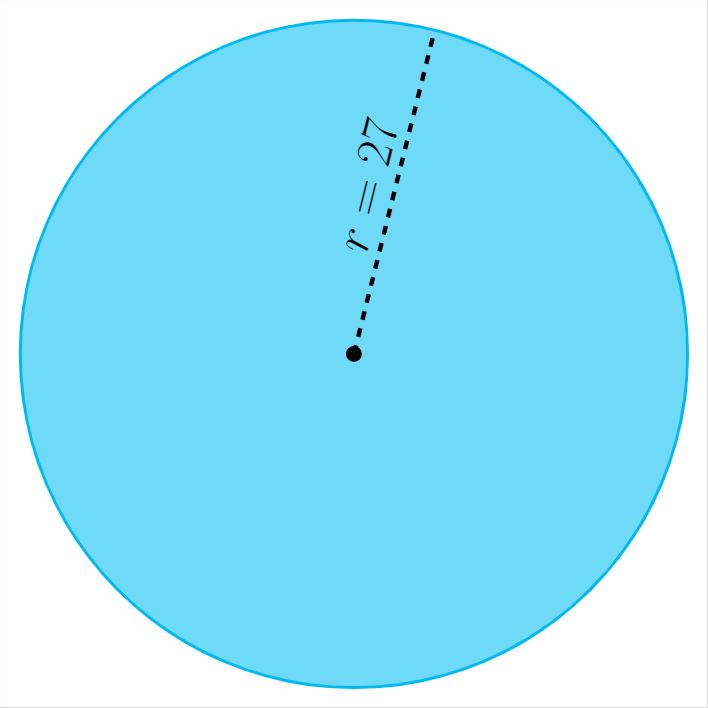
\includegraphics[width=0.85\linewidth]{mex_0006.png}\\
	%                   % Perímetro: \fillin[][0.3in] \quad Área: \fillin[][0.3in]
	%                   \part 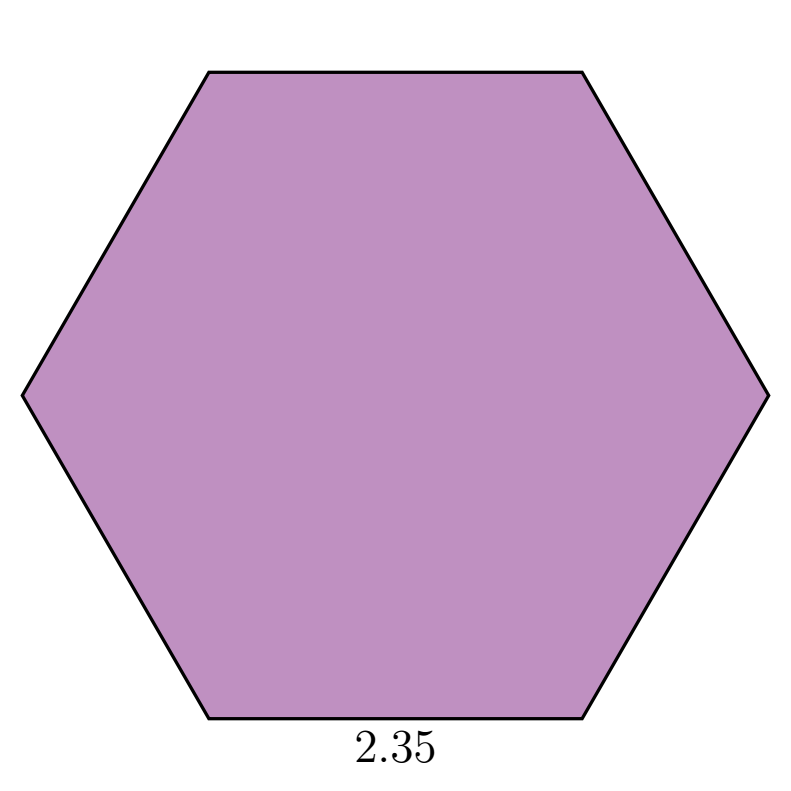
\includegraphics[width=0.85\linewidth]{mex_0007.png}\\
	%                   Perímetro: \fillin[][0.3in] \quad Área: \fillin[][0.3in]

	%                   \begin{solutionbox}{2cm}
	%                   \end{solutionbox}
	%                   % \part 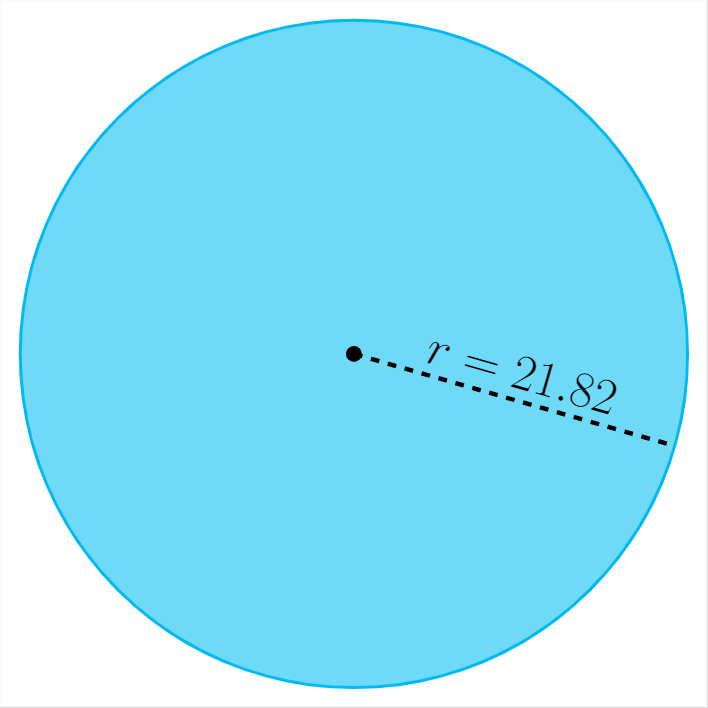
\includegraphics[width=0.85\linewidth]{mex_0008.png}\\
	%                   % Perímetro: \fillin[][0.3in] \quad Área: \fillin[][0.3in]
	%                   % \part 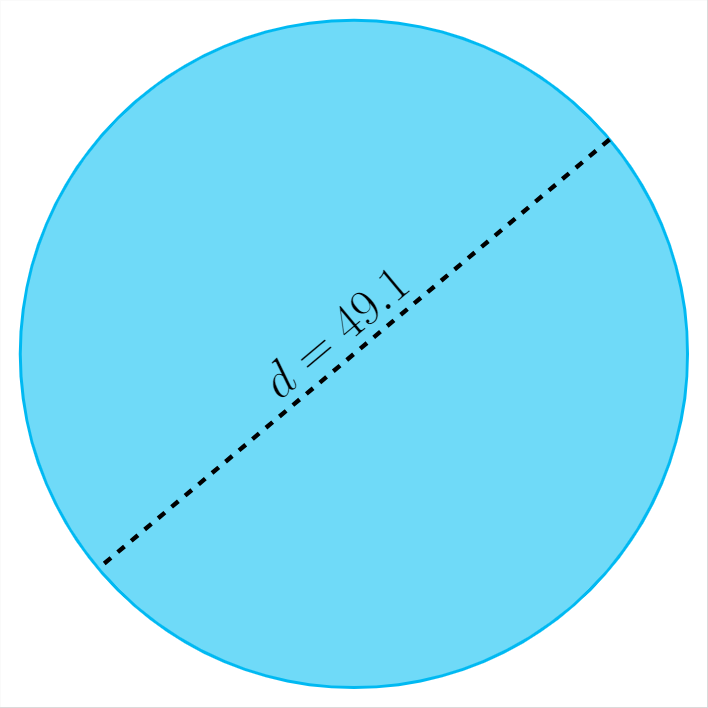
\includegraphics[width=0.85\linewidth]{mex_0009.png}\\
	%                   % Perímetro: \fillin[][0.3in] \quad Área: \fillin[][0.3in]
	%                   % \part 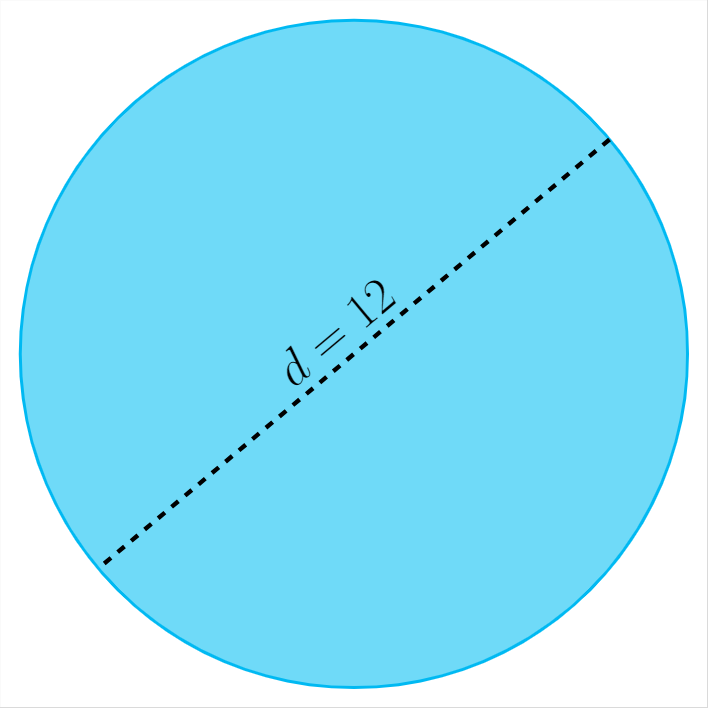
\includegraphics[width=0.85\linewidth]{mex_0010.png}\\
	%                   % Perímetro: \fillin[][0.3in] \quad Área: \fillin[][0.3in]
	%                   % \part 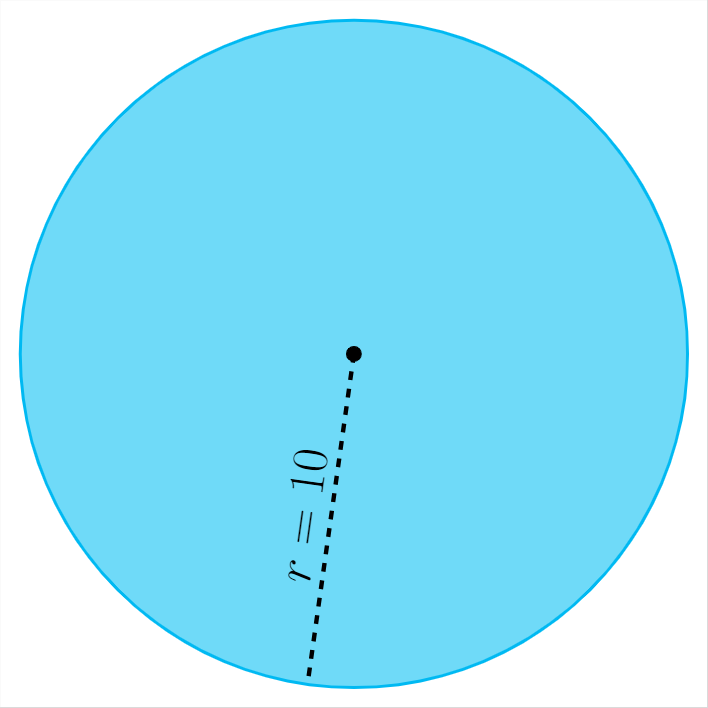
\includegraphics[width=0.85\linewidth]{mex_0011.png}\\
	%                   % Perímetro: \fillin[][0.3in] \quad Área: \fillin[][0.3in]
	%                   % \part 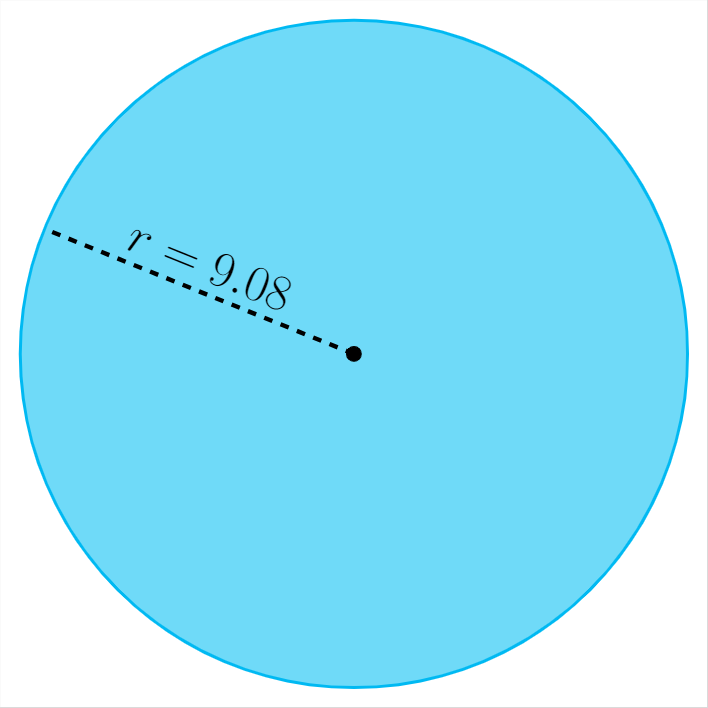
\includegraphics[width=0.85\linewidth]{mex_0012.png}\\
	%                   % Perímetro: \fillin[][0.3in] \quad Área: \fillin[][0.3in]
	%             \end{parts}
	%       \end{multicols}
	% }





	\question[6]{Responde a las siguientes preguntas:
		\begin{multicols}{2}
			\begin{parts}
				\part ¿Cuánto mide el ángulo exterior de un polígono de 6 lados? %\fillin[$60$][0in]

				\begin{solutionbox}{1.5cm}
					\[A_E=\frac{360^{\circ}}{n}=\frac{360^{\circ}}{6}=60^{\circ}\]
				\end{solutionbox}

				\part ¿Cuánto mide el ángulo central de un polígono de 20 lados? %\fillin[$18$][0in]

				\begin{solutionbox}{1.5cm}
					\[A_C=\frac{360^{\circ}}{n}=\frac{360^{\circ}}{20}=18^{\circ}\]
				\end{solutionbox}

			\end{parts}
		\end{multicols}
	}

	\newpage
	\question[4]{Calcula el valor del \textbf{ángulo} $x$:

		\begin{multicols}{3}
			\begin{parts}
				\part 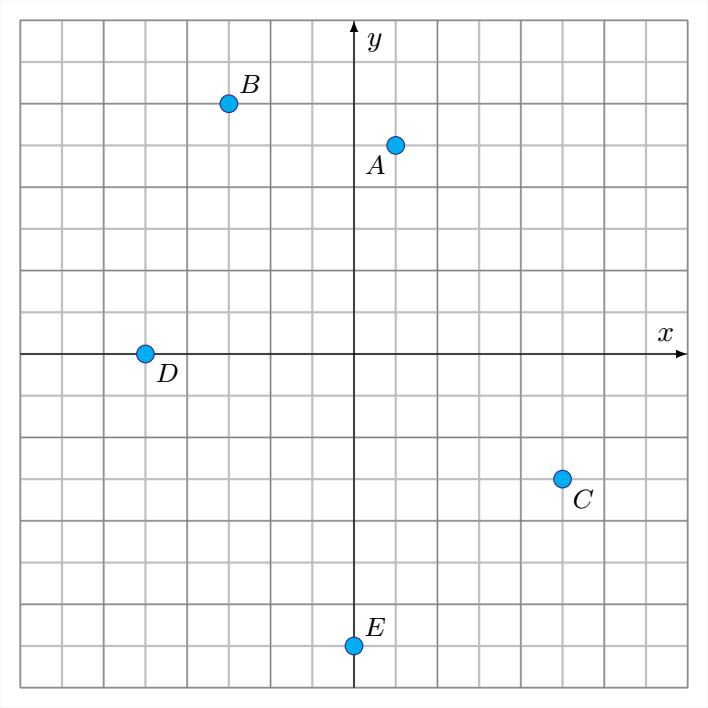
\includegraphics[width=.7\linewidth]{mex_0043.png}
				$x=$\fillin[$136^{\circ}$][0in]

				\part 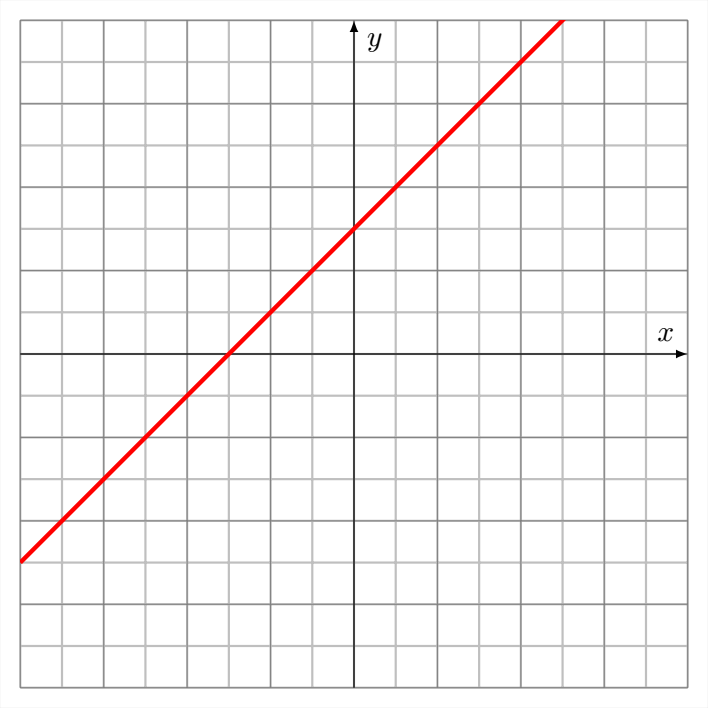
\includegraphics[width=.7\linewidth]{mex_0046.png}
				$x=$\fillin[$156^{\circ}$][0in]

				\part 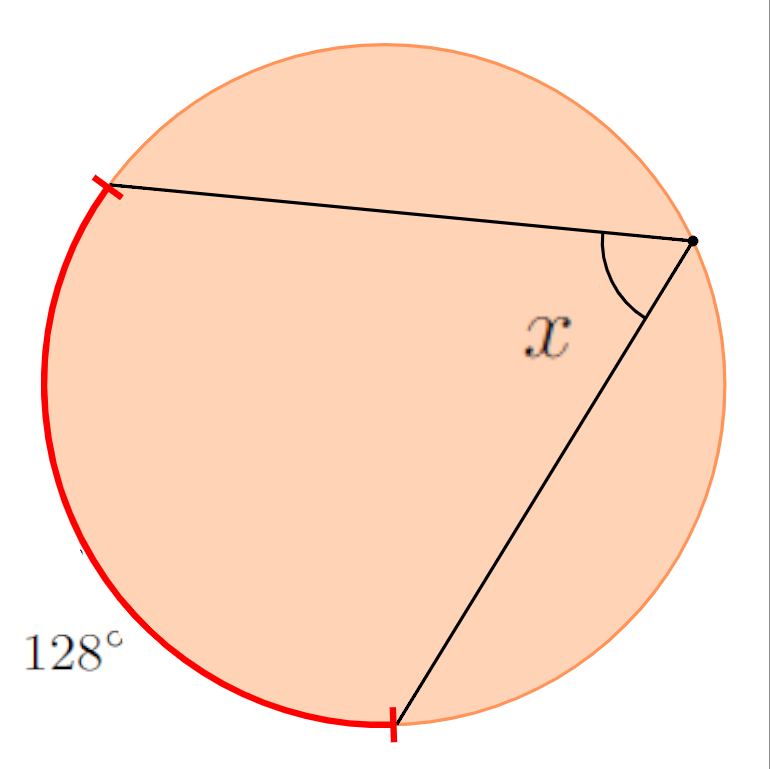
\includegraphics[width=.7\linewidth]{mex_0050.png}
				$x=$\fillin[$64^{\circ}$][0in]
			\end{parts}
		\end{multicols}
	}

	% \newpage

	\question[4]{Calcula el valor del \textbf{arco} $x$:

		\begin{multicols}{3}
			\begin{parts}
				\part 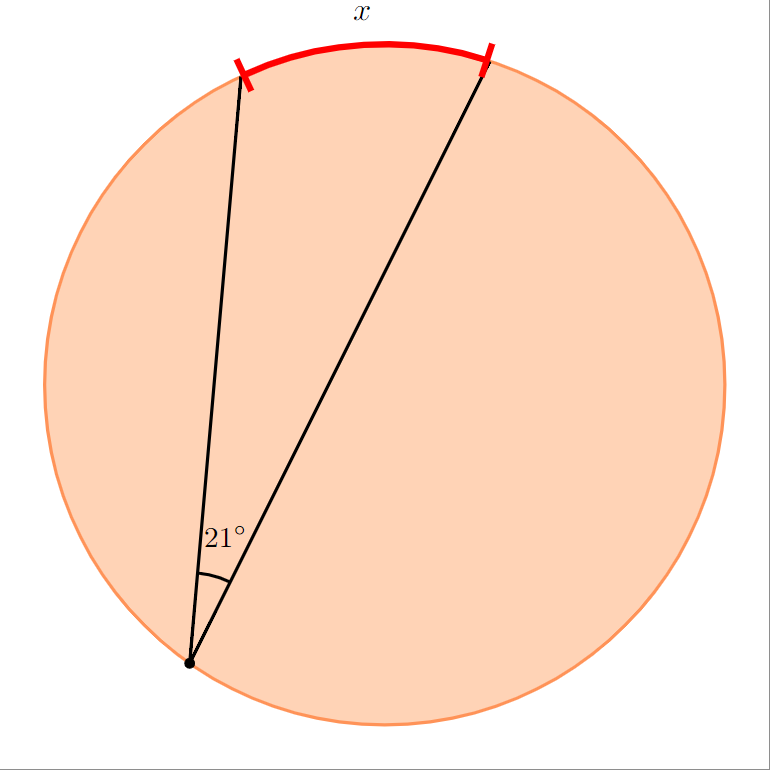
\includegraphics[width=.7\linewidth]{mex_0052.png}
				$x=$\fillin[$42$][0in]

				\part 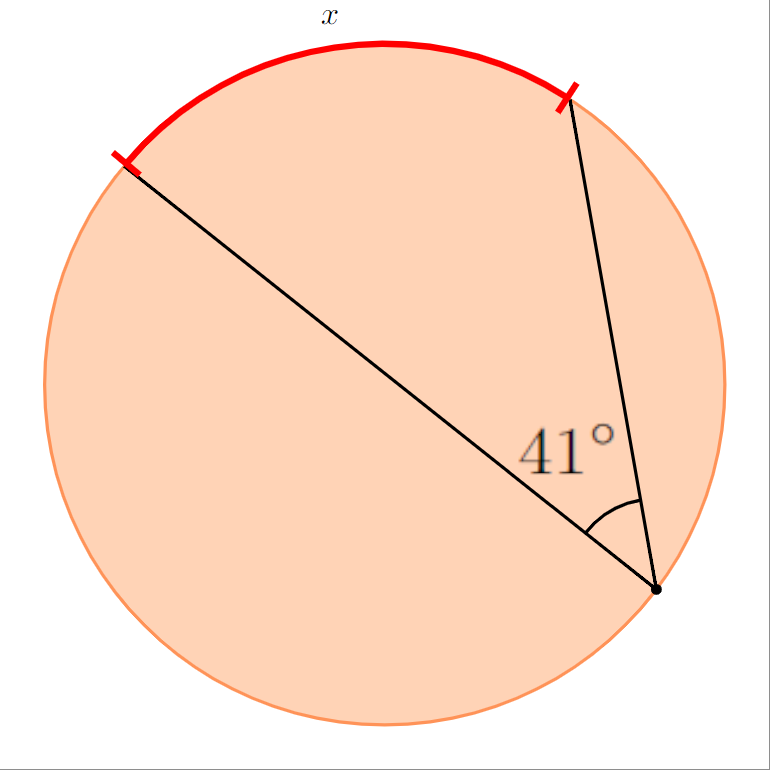
\includegraphics[width=.7\linewidth]{mex_0056.png}
				$x=$\fillin[$82$][0in]

				\part 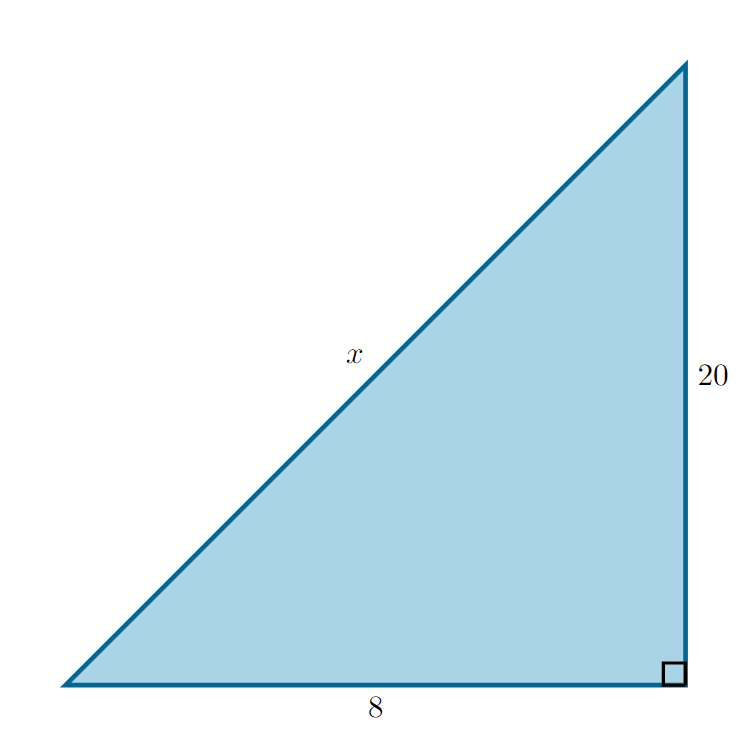
\includegraphics[width=.7\linewidth]{mex_0057.png}
				$x=$\fillin[$83$][0in]
			\end{parts}
		\end{multicols}
	}


	\question[4]{Calcula el área de cada uno de los siguientes sectores circulares:

		\begin{multicols}{3}
			\begin{parts}
				\part 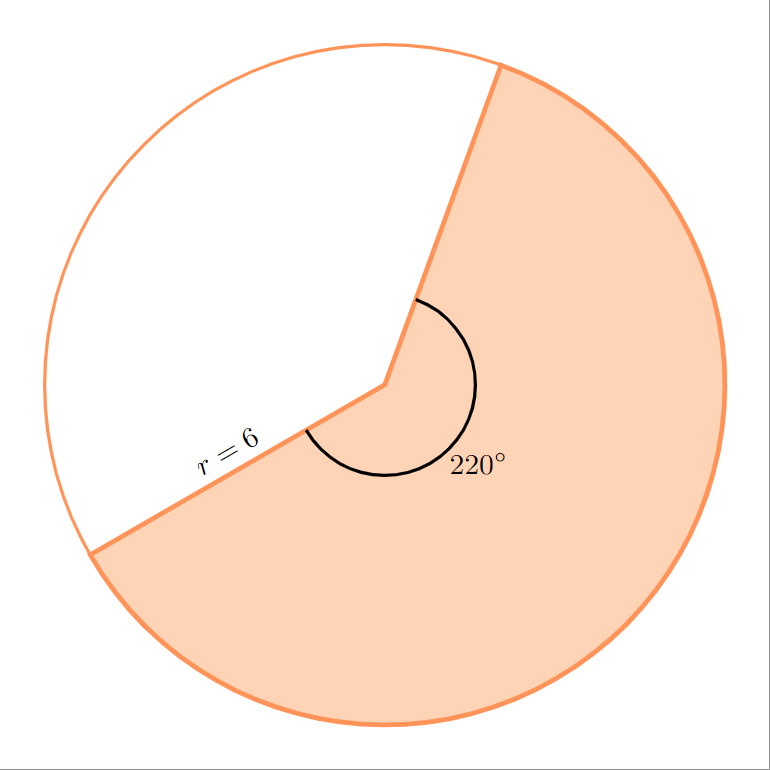
\includegraphics[width=.7\linewidth]{mex_0058.png}

				\begin{solutionbox}{2cm}
					\[ A=\pi r^2\left(\frac{x}{360}\right)\]
					$A=3.14(6)^2\left(\frac{220}{360}\right)=69.08$
				\end{solutionbox}

				\part 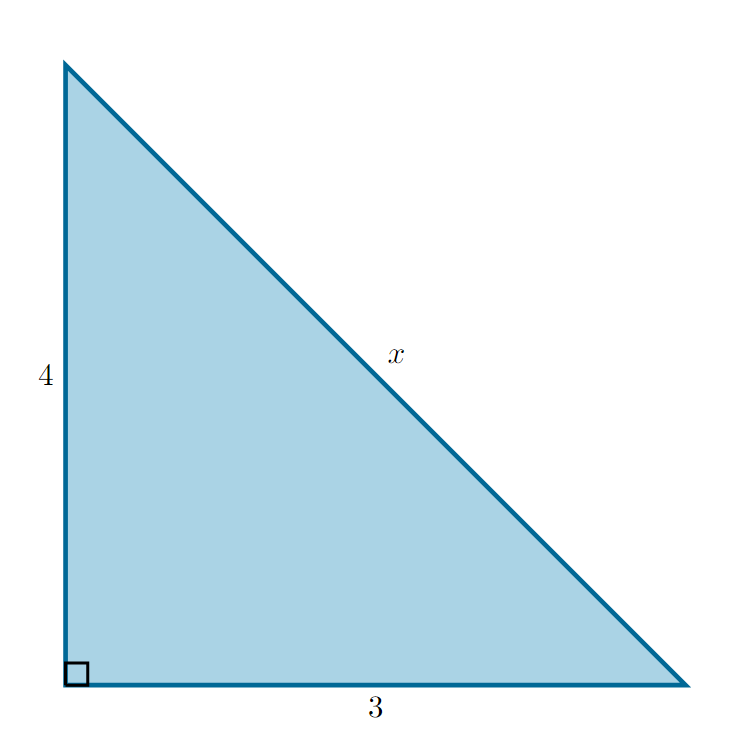
\includegraphics[width=.7\linewidth]{mex_0059.png}

				\begin{solutionbox}{2cm}
					\[ A=\pi r^2\left(\frac{x}{360}\right)\]
					$A=3.14(2)^2\left(\frac{104}{360}\right)=3.62$
				\end{solutionbox}

				\part 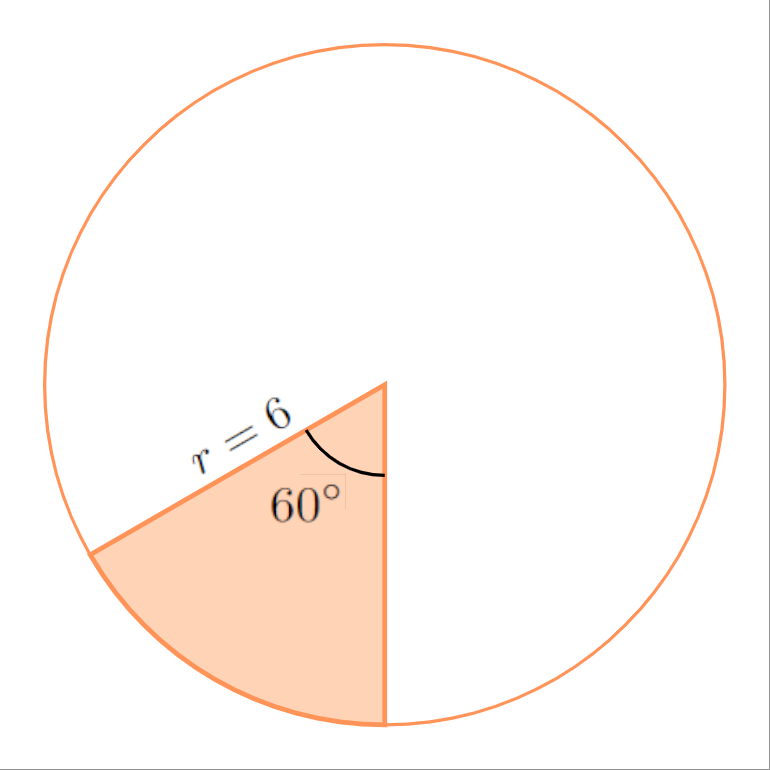
\includegraphics[width=.7\linewidth]{mex_0060.png}

				\begin{solutionbox}{2cm}
					\[ A=\pi r^2\left(\frac{x}{360}\right)\]
					$A=3.14(6)^2\left(\frac{60}{360}\right)=18.84$
				\end{solutionbox}

			\end{parts}
		\end{multicols}
	}






	\question[6]{Encuentra el perímetro de las siguientes figuras:

		\begin{multicols}{3}
			\begin{parts}
				\part 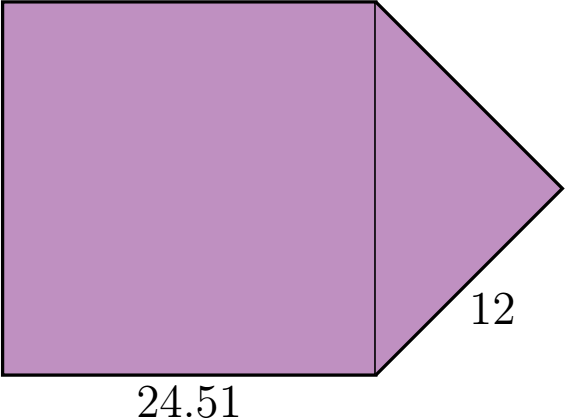
\includegraphics[width=.7\linewidth]{mex_0014.png}

				Perímetro: \\
				\fillin[$P=(3)24.51 + (2)12= 73.53+24=97.53$][0in]

				Área: \\
				\fillin[$A=24.51^2+\dfrac{12^2}{2}=600.74+72=672.74$][0in]

				\part 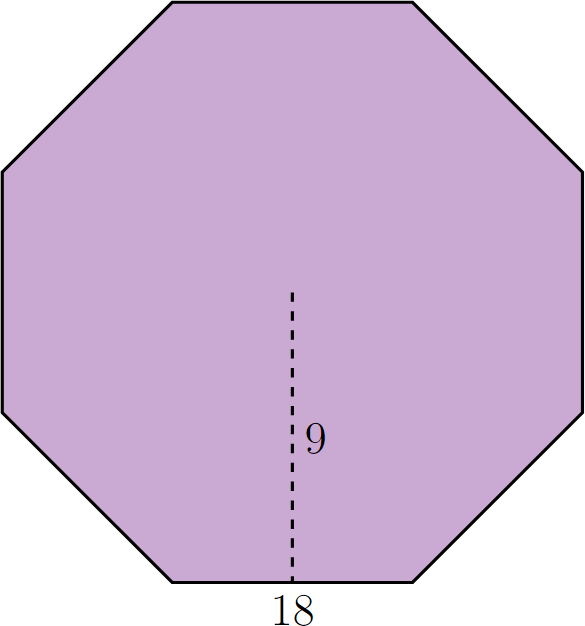
\includegraphics[width=.5\linewidth]{mex_0016.png}

				Perímetro: \\
				\fillin[$P=18\times 8 =144$][0in]

				Área: \\
				\fillin[$A=\dfrac{8\times 18 \times 9}{2}=648$][0in]

				\part 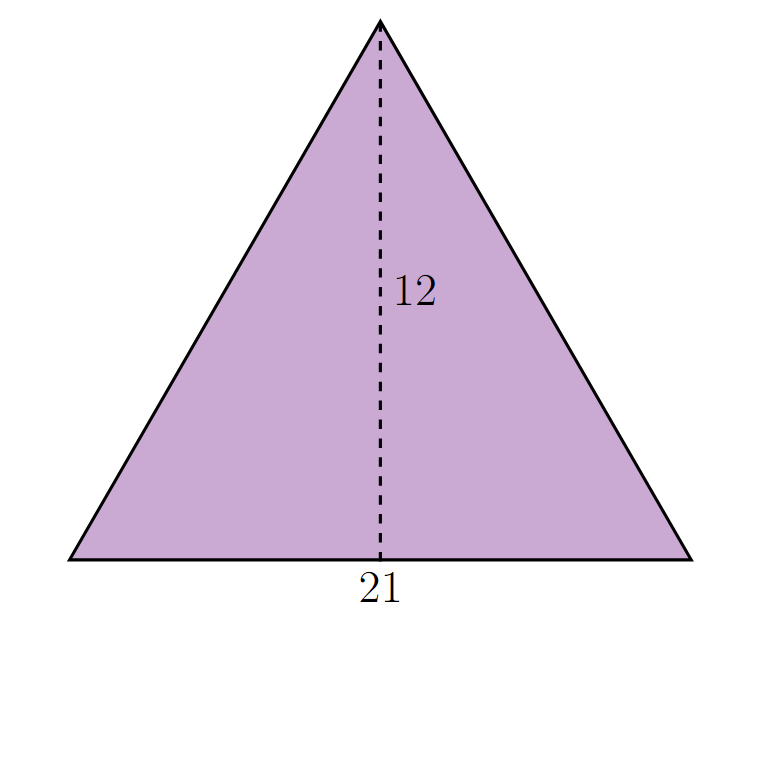
\includegraphics[width=.8\linewidth]{mex_0020.png}

				Perímetro: \\
				\fillin[$P=(2)61+(2)29=122+58=180$][0in]

				Área: \\
				\fillin[$A=61\times 29=1769$][0in]

			\end{parts}
		\end{multicols}
	}


	\question[6]{Calcula el \textbf{volumen}, el \textbf{área lateral} y el \textbf{área total} de las siguientes figuras:

		\begin{parts}
			\part Cilindro con altura $h=17$ cm y un radio $r=4$ cm.

			\begin{minipage}{.25\linewidth}
				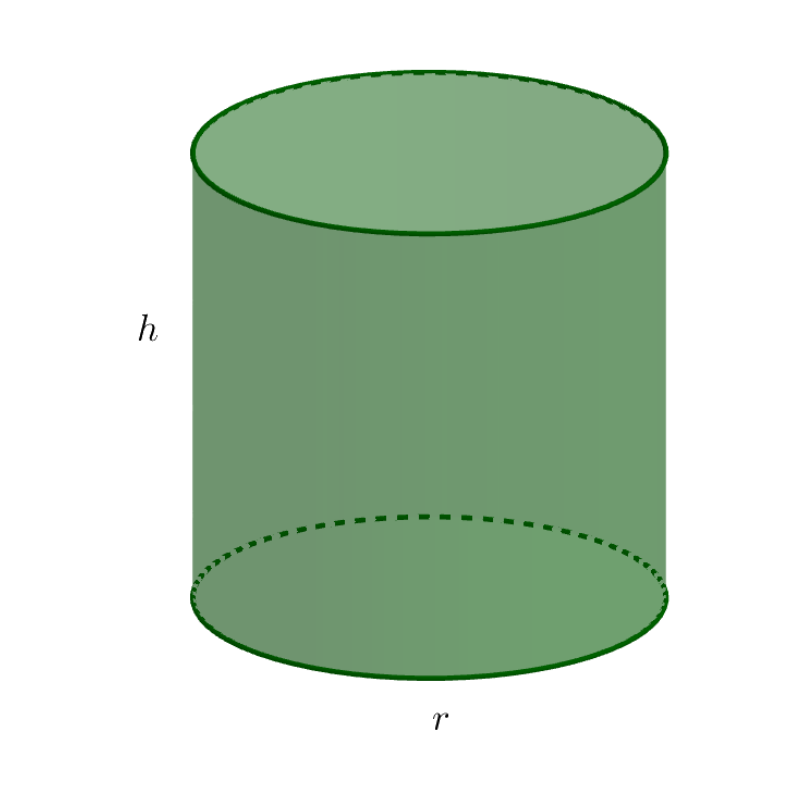
\includegraphics[width=0.8\linewidth]{mex_0024.png}
			\end{minipage}\hfill
			\begin{minipage}{.75\linewidth}
				Volumen:\\[-2em]
				\begin{solutionbox}{1.5cm}
					\[V=\pi r^2h=(3.14) 4^2\cdot 17= 857.12\]
				\end{solutionbox}

				A. Lateral:\\[-2em]
				\begin{solutionbox}{1.5cm}
					\[A_L=2\pi rh=2(3.14) 4\cdot 17= 2(3.14) 68=428.48\]
				\end{solutionbox}

				A. Total:\\[-2em]
				\begin{solutionbox}{1.5cm}
					\[A_T=A_L+2\pi r^2=428.48+2(3.14) 16=528.96\]
				\end{solutionbox}
			\end{minipage}

			\part Prisma octagonal de 19 cm de altura y su base es un octágono cuyos lados $l$ miden 7 cm y un apotema $a$ de 5 cm.

			\begin{minipage}{.25\linewidth}
				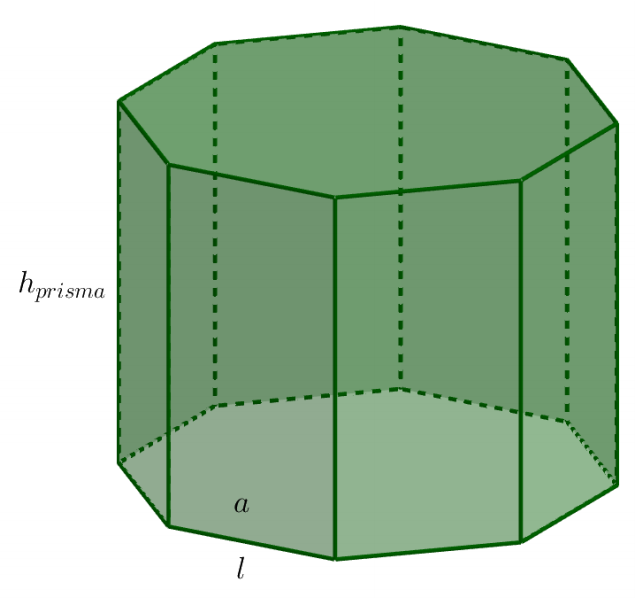
\includegraphics[width=0.8\linewidth]{mex_0025.png}
			\end{minipage}\hfill
			\begin{minipage}{.75\linewidth}
				Volumen:\\[-2em]
				\begin{solutionbox}{1.5cm}
					\[V=A_b\cdot h= \left(\dfrac{nla}{2}\right)h= \dfrac{8(7)5}{2}(19)=2660\]
				\end{solutionbox}

				A. Lateral:\\[-2em]
				\begin{solutionbox}{1.5cm}
					\[A_L=nlh=8(7)19= 1064\]
				\end{solutionbox}

				A. Total:\\[-2em]
				\begin{solutionbox}{1.5cm}
					\[A_T=A_L+2\dfrac{nla}{2}=A_L+nla=1064+280=1344\]
				\end{solutionbox}
			\end{minipage}
		\end{parts}
	}


	% \question[4]{Elige la expresión algebraica correcta para cada uno de los siguientes enunciados:

	%       \begin{multicols}{2}
	%             \begin{parts}
	%                   \part A un número se le resta 14.

	%                   \begin{oneparchoices}
	%                         \choice $a+14$
	%                         \CorrectChoice $a-14$
	%                         \choice $14a$
	%                         \choice $\dfrac{a}{14}$
	%                   \end{oneparchoices}

	%                   \part La suma de tres número diferentes

	%                   \begin{oneparchoices}
	%                         \choice $-xyz$
	%                         \choice $xyz$
	%                         \CorrectChoice $x+y+z$
	%                         \choice $x+y-z$
	%                   \end{oneparchoices}

	%                   \part El cubo de un número aumentado en 10

	%                   \begin{oneparchoices}
	%                         \choice $3x+10$
	%                         \choice $(x+10)^3$
	%                         \CorrectChoice $x^3+10$
	%                         \choice $x+10$
	%                   \end{oneparchoices}

	%                   \part El doble de la suma de un n\'umero con 2


	%                   \begin{oneparchoices}
	%                         \CorrectChoice $2(x+2)$
	%                         \choice $2x+2$
	%                         \choice $2+x$
	%                         \choice $(x+2)^2$
	%                   \end{oneparchoices}

	%                   \part La diferencia del triple de un n\'umero con 1.


	%                   \begin{oneparchoices}
	%                         \choice $3(1-a)$
	%                         \choice $3a+1$
	%                         \CorrectChoice $1-3a$
	%                         \choice $\dfrac{1}{3a}$
	%                   \end{oneparchoices}

	%                   \part Cinco novenos del cuadrado de un n\'umero.

	%                   \begin{oneparchoices}
	%                         \choice $\left(\dfrac{5}{9}x\right)^2$
	%                         \choice $\left(\dfrac{9}{5}x\right)^2$
	%                         \choice $5(9x^2)$
	%                         \CorrectChoice $\dfrac{5}{9}x^2$
	%                   \end{oneparchoices}

	%                   \part La mitad de la suma de un n\'umero con 3.


	%                   \begin{oneparchoices}
	%                         \choice $\frac{1}{2}x+3$
	%                         \CorrectChoice $\frac{x+3}{2}$
	%                         \choice $\frac{1}{2}+x+3$
	%                         \choice $\frac{x}{2}+3$
	%                   \end{oneparchoices}

	%                   \part La suma de la mitad de un n\'umero con 3.


	%                   \begin{oneparchoices}
	%                         \CorrectChoice $\frac{1}{2}x+3$
	%                         \choice $\frac{x+3}{2}$
	%                         \choice $\frac{1}{2}+x+3$
	%                         \choice $\frac{x}{2}+3$
	%                   \end{oneparchoices}


	%             \end{parts}
	%       \end{multicols}
	% }

	\question[6]{Resuelve los siguientes problemas:

		\begin{multicols}{2}
			\begin{parts}
				\part Calcula la altura de un prisma que tiene como área de la base 6 m$^2$ y 99 m$^3$ de capacidad.

				\begin{solutionbox}{3cm}
					Ya que el volumen de un prisma es: $V=A_b\cdot h$, entonces la altura del prisma es: \[h=\dfrac{V}{A_b}=\dfrac{99}{6}=16.5\text{m}\]
				\end{solutionbox}

				\part ¿Cuál es el perímetro de un campo de fútbol que mide 95.12 metros de largo y 45.27 metros de ancho?

				\begin{solutionbox}{3cm}
					El perímetro de un rectángulo es: $P=2(l+a)$ entonces el perímetro del campo de fútbol es: \[P=2(95.12+45.27)=280.78\text{m}\]
				\end{solutionbox}

			\end{parts}
		\end{multicols}
	}

	\newpage
	\question[3]{Encuentra el área de las siguientes figuras:

		\begin{multicols}{4}
			\begin{parts}
				\part 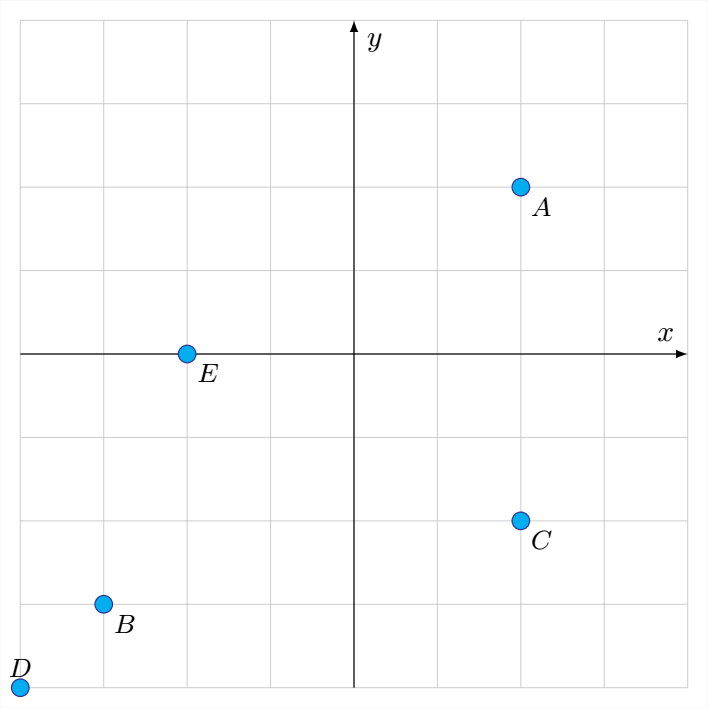
\includegraphics[width=.85\linewidth]{mex_0036.png}\\[0.5em]
				Área: \fillin[$x^2-6x+9$][0in]

				\part 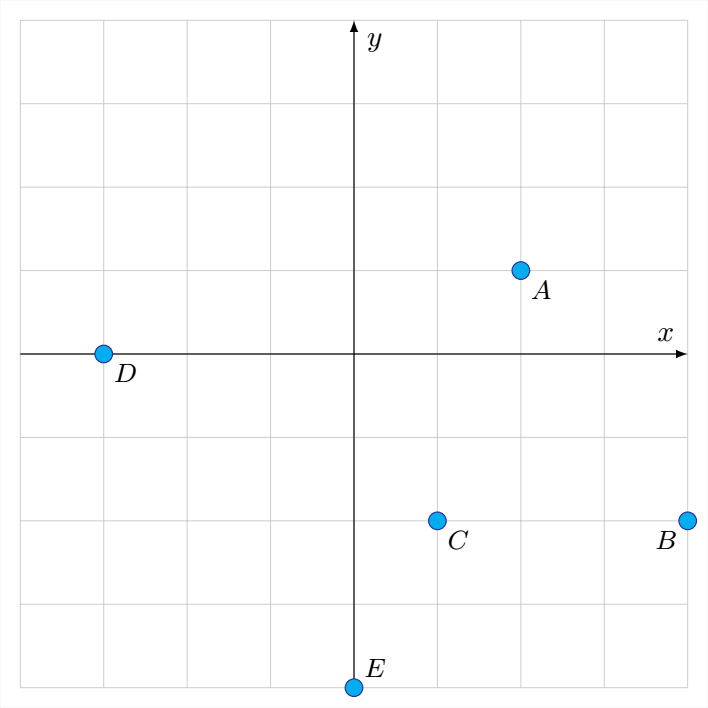
\includegraphics[width=1.2\linewidth]{mex_0037.png}\\[0.5em]
				Área: \fillin[$10x^2-50x$][0in]

				\part 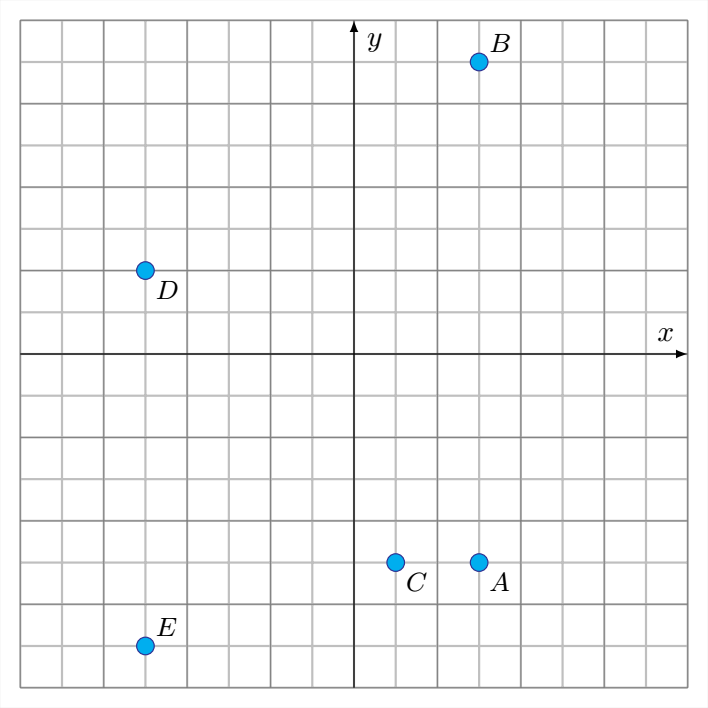
\includegraphics[width=1.2\linewidth]{mex_0038.png}\\[0.5em]
				Área: \fillin[$x^2+7x-30$][0in]

				\part 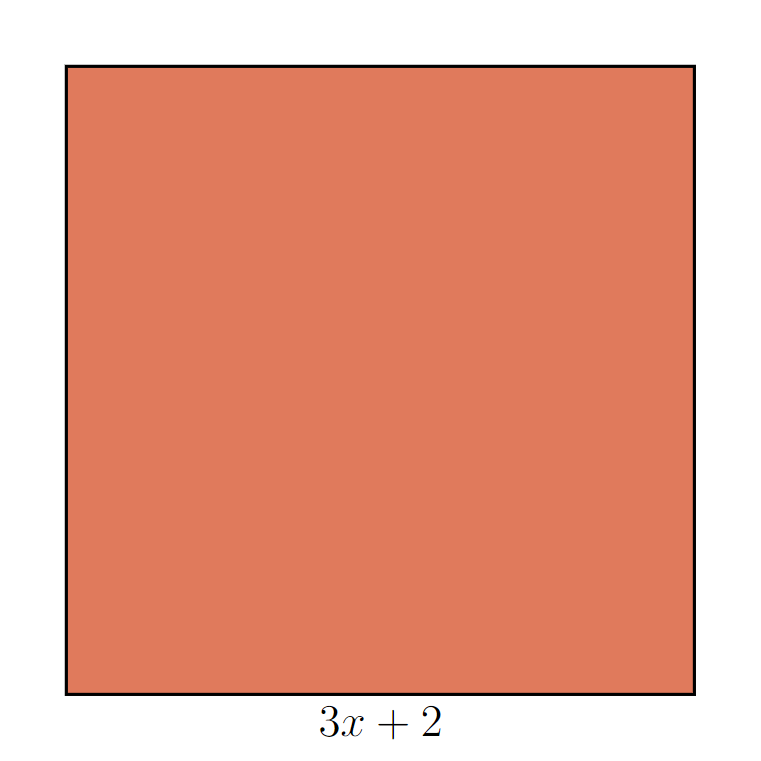
\includegraphics[width=.85\linewidth]{mex_0041.png}\\[0.5em]
				Área: \fillin[$9x^2+12x+4$][0in]
			\end{parts}
		\end{multicols}
	}



	\question[6]{Resuelve las siguientes sumas de monomios y polinomios:

		\begin{multicols}{2}
			\begin{parts}
				\part $(b+9c)+(-2b-3c)+(2a-4b-5c)=$ \\ \fillin[$2a-5b+c$][0in]
				\part $(a+b+c)+(2a+2b+2c)=$ \\ \fillin[$3a+3b+3c$][0in]
			\end{parts}
		\end{multicols}
	}


	\question[6]{Resuelve las siguientes restas de monomios y polinomios:

		\begin{multicols}{2}
			\begin{parts}
				\part $(8a-b-5c)-(-2a+5b+3c)=$  \\ \fillin[$10a-6b-8c$][0in]
				\part $(a+2b+3c)-(a-b+c)-(3a-4b-c)=$  \\\fillin[$-3a+7b+3c$][0in]
			\end{parts}
		\end{multicols}
	}



	\question[6]{Resuelve las siguientes operaciones convinadas:
		\begin{multicols}{2}
			\begin{parts}
				\part $2(x-3y+7)-5(3x+4y-7)=$ \\ \fillin[$-13x-26y+49$][0in]
				\part $2(8x)+5(-x+7)=$ \\\fillin[$11x+35$][0in]                  \end{parts}
		\end{multicols}
	}

	\question[6]{Realiza las siguientes operaciones con exponentes:
		\begin{multicols}{3}
			\begin{parts}
				\part $7x^2\cdot 3x^4 \cdot x^2=$  \fillin[$21x^8$][0in]

				\part $\dfrac{x^{4}yz}{x^{3}yz}=$  \fillin[$x$][0in]

				\part $\left(a^2 b^4 c^{3} \right)^8=$  \fillin[$a^{16}b^{32}c^{24}$][0in]

			\end{parts}
		\end{multicols}
	}

	\question[6]{Realiza la siguientes multiplicaciones de polinomios:

		\begin{multicols}{2}
			\begin{parts}
				% \part $(x-3)(x^2-5x+4)=$ \fillin[$x^3-8x^2+19x-12$][0in]
				% \part $(2a+3b)(4x+3y)=$ \fillin[$8ax+6ay+12bx+9by$][0in]
				% \part $(x+1)(x+2)(x+3)=$ \fillin[$x^3+6x^2+11x+6$][0in]
				% \part $(x+5)(2x^2+3x-7)=$ \fillin[$2x^3+13x^2+8x-35$][0in]
				\part $(x-1)(x+1)(x^2+1)=$ \fillin[$x^4-1$][0in]

				\begin{solutionbox}{2cm}
				\end{solutionbox}
				% \part $(x+5)(x^2+2x-3)=$ \fillin[$x^3+7x^2+7x-15$][0in]
				% \part $(x+-3(x-3)(x-2)=$ \fillin[$x^3-8x^2+21x-18$][0in]
				\part $(x+y)(x^2-xy+y^2)=$ \fillin[$x^3+y^3$][0in]

				\begin{solutionbox}{2cm}
				\end{solutionbox}
			\end{parts}
		\end{multicols}
	}

	\newpage
	% \section*{\ifprintanswers{Sistema de unidades}\else{}\fi}
	% \subsection*{\ifprintanswers{Unidades de longitud y masa}\else{}\fi}
	\question[4]{Convierte las siguientes unidades de longitud y de masa como se te pide:

		\begin{multicols}{2}
			\begin{parts}
				\part  54 metros ($m$) a hectómetros ($Hm$).       \\ \fillin[$54\divisionsymbol 10 \divisionsymbol 10=0.54$][0in]

				\part  6.5 gramos ($g$) a hectogramos ($Hg$).	   \\ \fillin[$6.5\divisionsymbol 10 \divisionsymbol 10=0.065$][0in]

			\end{parts}
		\end{multicols}
	}

	% \subsection*{\ifprintanswers{Unidades de capacidad}\else{}\fi}
	\question[4]{Convierte las siguientes unidades de capacidad como se te pide:

		\begin{multicols}{2}
			\begin{parts}
                        \part 4.8  decímetros cúbicos ($dm^3$) a litros ($L$).	  \\ \fillin[$4.8=4.8$][0in]
                        \part 567  milímetros cúbicos ($mm^3$) a litros ($L$).	  \\ \fillin[$567 \divisionsymbol 1000 \divisionsymbol 1000=0.000567$][0in]
			\end{parts}
		\end{multicols}

	}
	% \subsection*{\ifprintanswers{Unidades de área y volumen}\else{}\fi}
	\question[5]{Convierte las siguientes unidades de área y volumen como se te pide:

		% \begin{multicols}{2}
			\begin{parts}
                        \part  8.8 metros cúbicos ($m^3$) a milímetros cúbicos ($mm^3$) \\ \fillin[$8.8\times 1000 \times 1000 \times 1000=8800000000$][0in] \\[3em]
				% \columnbreak%

				\part  18 decámetros cúbicos ($Dm^3$) a centímetros cúbicos ($cm^3$)	\\ \fillin[$18\times 1000 \times 1000 \times 1000=18000000000$][0in]

			\end{parts}
		% \end{multicols}
	}
\end{questions}
\end{document}